\documentclass[a4paper,12pt,twoside]{article}
\usepackage[T1,T2A]{fontenc}
\usepackage[utf8]{inputenc}


\usepackage{graphicx}
\usepackage{blindtext}
\usepackage{ mathrsfs }
\usepackage[russian,english]{babel}
\usepackage{enumitem}
\usepackage[english,russian]{babel}
\usepackage{amsmath}
\usepackage[section]{placeins}
\usepackage{amssymb}
\usepackage[top=20mm, bottom=20mm, left=20mm, right=20mm]{geometry}


	\title{Применение нейроных сетей для апроксимации\\ криптографического примитива ГОСТ 28147}
	
	
\begin{document}
	\begin{center}
		{МИНИСТЕРСТВО  ОБРАЗОВАНИЯ  РЕСПУБЛИКИ  БЕЛАРУСЬ\\
			БЕЛОРУССКИЙ ГОСУДАРСТВЕННЫЙ УНИВЕРСИТЕТ\\
			ФАКУЛЬТЕТ ПРИКЛАДНОЙ МАТЕМАТИКИ И ИНФОРМАТИКИ} \\
		{Кафедра математичекого моделирования и анализа данных}
		
	\end{center}
	
	\begin{center}
		\bigskip
		\bigskip
		\bigskip
		\bigskip
		\textbf{Отчёт\\ о прохождении производственной практики\\ для специальности \\
			1-31 81 12«Прикладной компьютерный анализ данных»}
	\end{center}
	
	\bigskip
	\bigskip
	\bigskip
	\bigskip
	\bigskip
	
	\hfil\hfil\hfil\hfil	\textbf{магистранта 2 года обучения}\\
	\bigskip
	\hfil\hfil\hfil\hfil\hfil	\textit{Деркача Максима Юрьевича}\\
	\bigskip
	
	\hfil\hfil\hfil\hfil	\textbf{Руководитель практики от кафедры}\\
	
	\hfil\hfil\hfil\hfil\hfil	\textit{чл.-корр. НАН Беларуси},
	
	\hfil\hfil\hfil\hfil	\textit{доктор физ.-мат. наук, профессор}
	
	\hfil\hfil\hfil\hfil\hfil	\textit{Харин Юрий Семенович}\\

	
	\hfil\hfil\hfil\hfil	\textbf{Руководитель практики от организации}
	
	\bigskip
	\hfil\hfil\hfil\hfil\hfil	\textit{Пьянов Владислав Сергеевич}\\
	
	\bigskip
	\bigskip
	\bigskip
	\bigskip
	\bigskip
	\bigskip
	\bigskip
	\bigskip
	\bigskip
	
	\begin{center}
		Минск, 2019
	\end{center}
	
	
	\newpage
	
	{
		\renewcommand{\contentsname}{Оглавление}
		\tableofcontents
	}
	
	\newpage
	\section{Введение}
	\bigskip
	
	Проблема защиты информации затрагивает практически все сферы деятельности человека. Среди способов защиты информации важнейшим считается криптографический [1]. 
	
	Нейронная криптография - это раздел криптографии, посвященный анализу применения стохастических алгоритмов, особенно алгоритмов искусственных нейронных сетей, для использования в шифровании и криптоанализе.[2] Существуют решения, построенные на основе искусственных нейронных сетей, позволяющие обеспечить доступность данных [3].
	
	Архитектура искусственных нейронных сетей позволяет эффективно проводить работы по распознаванию образов и классификации множества объектов по любым признакам. Кроме того, благодаря хорошо продуманному алгоритму обученные нейронные сети могут достигать чрезвычайно высоких уровней точности. 
	
	Основной целью практики являлось построение нейронных сетей, для апроксимации элементарных преобразований из алгоритма шифрования ГОСТ 28147-89, проведение компьютерных экспериментов и проведение анализа полученных результатов. 
	
	\newpage
	
	\section{Описание математических моделей}
	
	\bigskip
	\noindent Опишем однотактовое преобразование шифрования ГОСТ 28147-89.
	\bigskip
	
	$Y = g(X, K) = g(X_1 || X_2, K) \equiv (S[X_1 \boxplus K] \ll 11) \oplus X_2 || X_1,$ где
	
	$X \in V_{64}$ - вектор входных данных,
	
	$Y \in V_{64}$ - выходные данные,
	
	$K \in V_{32}$ - ключ,
	
	$S$ - стандартный S-блок из ГОСТ-28147.
	
	\bigskip
	\noindent 
	Определим следущие математичские модели (элементы преобразования), для которых в дальнейшем будут ппостроены нейронные сети и проведены компьютерные эксперименты.
	
	\begin{enumerate}
	\item 
	$Y_{g_0} = g_0(x) = g_1(x_1 || x_2)\equiv x_1 \oplus x_2,$ где
	
	$x \in V_{8}$ - вектор входных данных,
	
	$x_1, x_2 \in V{4}$ - левая и правая часть входного вектора,
	
	$Y_{g_0} \in V_{4}$ - выходные данные модели $g_0$;
	\bigskip
		
	\item 
	$Y_{g_1} = g_1(x) = g_1(x_1 || x_2, k) \equiv S[x_1] \oplus x_2,$ где
	
	 $x \in V_{8}$ - вектор входных данных,
	 
	 $x_1, x_2 \in V{4}$ - левая и правая часть входного вектора,
	 
	 
	 $Y_{g_1} \in V_{4}$ - выходные данные модели $g_1$,
	 
	 $S$ - стандартный S-блок из ГОСТ-28147;
	\bigskip
	
	\item 
	$Y_{g_2} = g_2(x) = g_2(x_1 || x_2, k) \equiv S[x_1 \boxplus k] \oplus x_2,$ где
	
	$x \in V_{8}$ - вектор входных данных,
	
	$x_1, x_2 \in V{4}$ - левая и правая часть входного вектора,
	
	$k \in V_{4}$ - некоторый неизвестный постоянный в эксперименте ключ (4-ех битный ключ),
	
	$Y_{g_2} \in V_{4}$ - выходные данные модели $g_2$,
	
	$S$ - стандартный S-блок из ГОСТ-28147.


	%\item 
	%$Y_{g3} = g(X) = g(X_1 || X_2, K) \equiv (S[X_1 \boxplus K] \ll 11) \oplus X_2,$ где

%	$X \in V_{64}$ - вектор входных данных,
%
%	$K \in V_{32}$ - некоторый неизвестный ключ,
%	
%	$Y_{g3} \in V_{32}$ - выходные данные модели $g_3$.
	\end{enumerate}
	
	\bigskip
	\noindent Опишем определеные ранее модели как частные случаи однотактового преобразования шифрования ГОСТ 28147-89:
	\begin{enumerate}
		\item Модель $g_0$ является однотактовым преобразованием  шифрования ГОСТ 28147-89, при слудеующих условиях:
			\begin{itemize}
			\item S-блок - прямая таблица подстановки (подстановка при которой исходное значение переходит в такое же знанчение).
			\item $K = 0^{32}$.
			\item Отсутствует сдвиг влево на 11 бит.
			\item Рассмотриваются только первые 4-бита $X_1, X_2, Y$.
			\end{itemize}
		\item Модель $g_1$ является однотактовым преобразованием  шифрования ГОСТ 28147-89, при слудеующих условиях:
		\begin{itemize}
			\item S-блок - стандартный S-блок из ГОСТ-28147.
			\item $K = 0^{32}$.
			\item Отсутствует сдвиг влево на 11 бит.
			\item Рассмотриваются только первые 4-бита $X_1, X_2, Y$.
		\end{itemize}
		\item Модель $g_1$ является однотактовым преобразованием  шифрования ГОСТ 28147-89, при слудеующих условиях:
		\begin{itemize}
			\item S-блок - стандартный S-блок из ГОСТ-28147.
			\item $K$ - некоторый неизвестный постоянный в эксперименте ключ.
			\item Отсутствует сдвиг влево на 11 бит.
			\item Рассмотриваются только первые 4-бита $X_1, X_2, Y$.
		\end{itemize}
	\end{enumerate}
	
	\newpage
	\section{Описание используемых нейронных сетей}	
	\bigskip
	\noindent Для решения поставленных задач использовались следующие нейронные сети:
	
	\begin{enumerate}
		\item Однослойная нерйоная сеть;	
		\item Многослойная нерйоная сеть с одним скрытым слоем, с переменным количеством нейронов на скрытом слое;
		\item Многослойная нерйоная сеть с двумя скрытым слоями, c 
		переменным количеством нейронов на скрытых слоях.
	\end{enumerate}
	
	
	\noindent Точность построенной модели к реальной оценивалась использовалось расстояние Хэмминга:
	$w(y, \hat{y}) = \sum_{i=1}^{j} y_i \oplus \hat{y}_i$, где $y_i \in V_j$.
	\bigskip
	
	\noindent Для оценки точности проведенного эксперимента использовалось следующая функция:
	$\hat{f} =L - \dfrac{1}{T_e}\sum_{j=1}^{T_e}w(y^{(j)}, \hat{y^{(j)}})$,
	где $L$ - количество бит в выходных данных оцениваемой модели. 

	\bigskip
	\noindent Компьютерные эксперименты проводились на следующих данных:
	\begin{enumerate}
		\item Обучающая выборка $T_o=18 * 10^3$ пар $(x, x_1)$;
		\item Экзаменационная выборка $T_e=2 * 10^3$ пар $(x, x_1)$.
	\end{enumerate}
	
	
	\newpage
	\section{Результаты компьютерных экспериментов}
	
	\begin{figure}[htb!]
	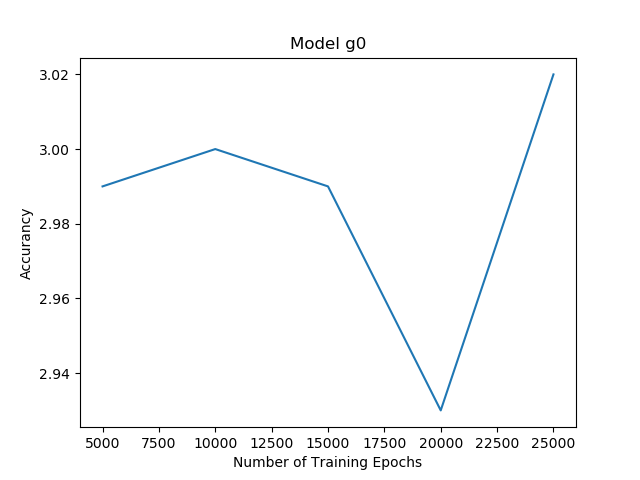
\includegraphics[width=0.8\linewidth]{report_1/acc_g0_0.png}
	
	График точности построенной однослойной неройной сети модели $g_0$ от количества итераций обучения.
	
	
	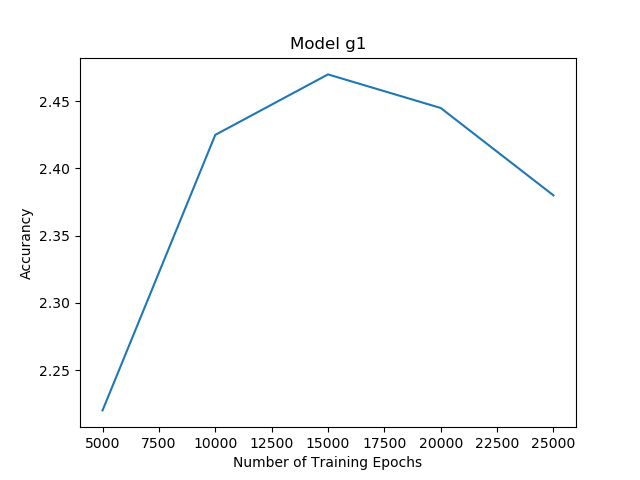
\includegraphics[width=0.8\linewidth]{report_1/acc_g1_0.png}
	
	График точности построенной однослойной неройной сети модели $g_1$ от количества итераций обучения.
	
	\end{figure}

	\begin{figure}[h!]
	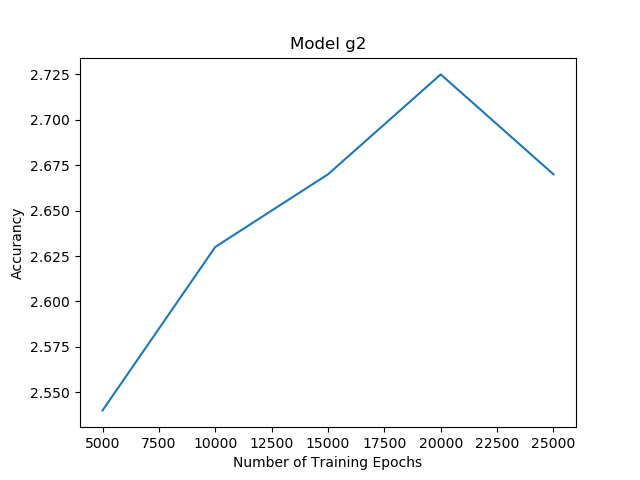
\includegraphics[width=0.9\linewidth]{report_1/acc_g2_0.png}
	
	График точности построенной однослойной неройной сети модели $g_2$ от количества итераций обучения.
	
	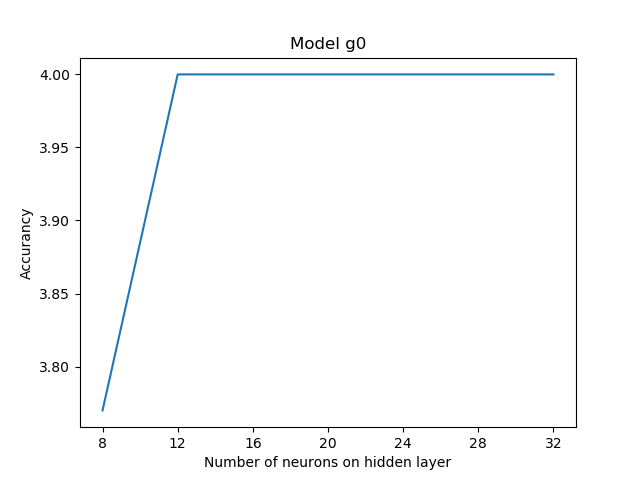
\includegraphics[width=0.9\linewidth]{report_1/acc_g0_1.png}
	
	График точности построенной неройной сети модели $g_0$ от кол-ва нейронов на скрытом слое.
	\end{figure}
	
	\begin{figure}[h!]
	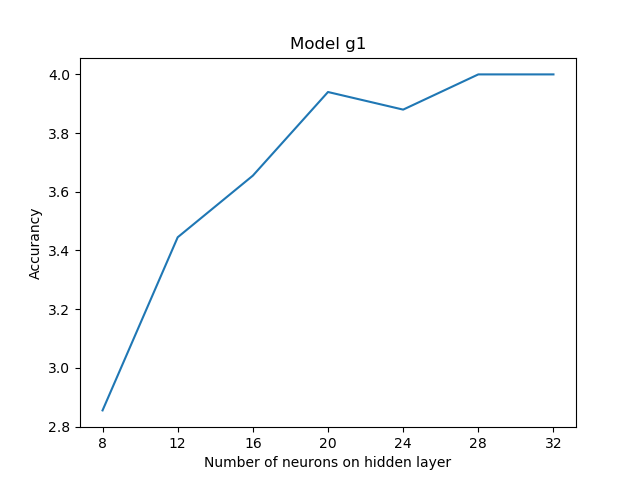
\includegraphics[width=0.9\linewidth]{report_1/acc_g1_1.png}
	
	График точности построенной неройной сети модели $g_1$ от кол-ва нейронов на скрытом слое.

	
	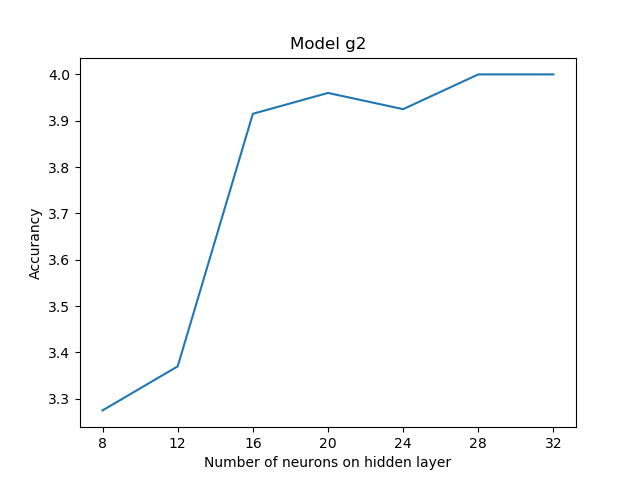
\includegraphics[width=0.9\linewidth]{report_1/acc_g2_1.png}
	
	График точности построенной неройной сети модели $g_2$ от кол-ва нейронов на скрытом слое.
	\end{figure}

	\begin{figure}[h!]
	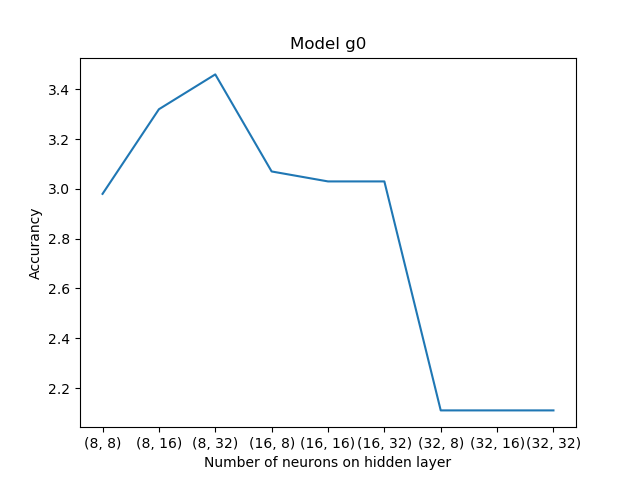
\includegraphics[width=0.9\linewidth]{report_1/acc_g0_2.png}
	
	График точности построенной неройной сети модели $g_0$ от кол-ва нейронов на скрытых слоях.
	
	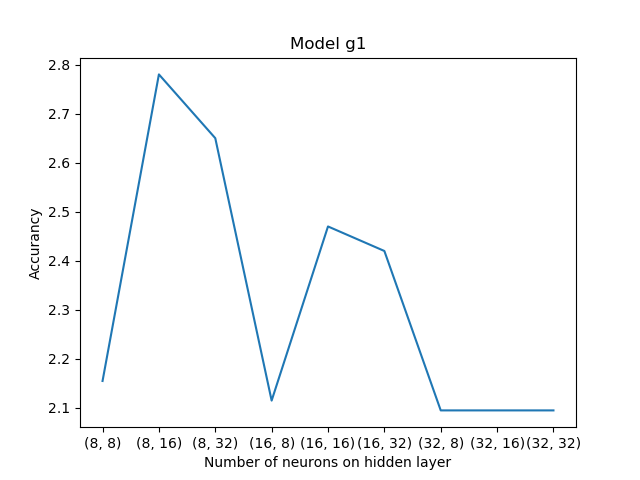
\includegraphics[width=0.9\linewidth]{report_1/acc_g1_2.png}
	
	График точности построенной неройной сети модели $g_1$ от кол-ва нейронов на скрытых слоях.
	\end{figure}
	
	\begin{figure}[htb!]
	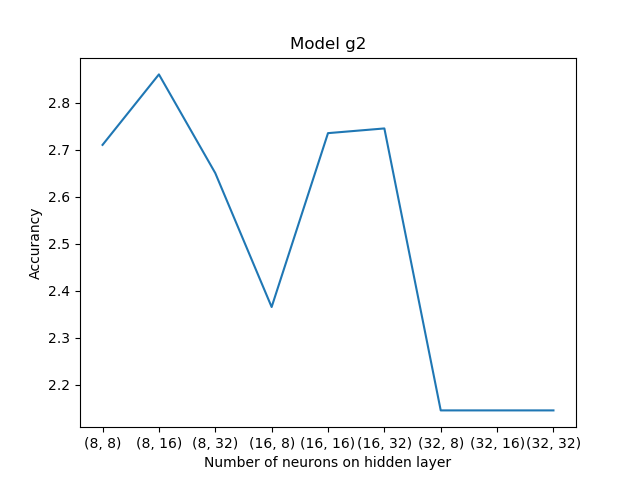
\includegraphics[width=0.9\linewidth]{report_1/acc_g2_2.png}
	
	График точности построенной неройной сети модели $g_2$ от кол-ва нейронов на скрытых слоях.
	\end{figure}

	\section{Анализ результатов}
	\bigskip
	Исходя из полученных результатов можно сделать выводы, что нейронная сеть с одним скрытым слоем наиболее точно аппроксимирует построенные модели.
	
	\bigskip
	
	\noindent  И для аппроксимации однотактового преобразования шифрования ГОСТ 28147-89, можно воспользоваться моделью $g_2$ и нейронной сетью, построенной для это модели.
	
	\bigskip
	
	\noindent  Метод построение нейронной сети для аппроксимации однотактового преобразования шифрования ГОСТ 28147-89:
	\begin{enumerate}
	\item Входной вектор $X_1 \in V_{64}$ разбиваем на блоки длинной 4 бита ($x_1^{i}$).
	
	\item Входной вектор $X_2 \in V_{64}$ сдвигаем вправо на 11 бит и разбиваем на блоки длинной 4 бита ($x_2^{i}$).
	
	\item Выходной вектор $Y$ также сдвигаем вправо на 11 бит разбиваем на блоки длинной 4 бита ($y^{i}$).
	
	\item Для каждого набора блоков $x_1^{i}, x_2^{i}, y^{i}, i=1,..8$, обучаем нейронную сеть.
	
	\item Полученный набор нейронных сетей можно использовать для аппроксимации однотактового преобразования шифрования ГОСТ 28147-89.
	
	\end{enumerate}
	\bigskip
	
	\noindent Для данного метода были проведены компьютерные эксперименты, используя нейронные сети с одним скрытым слоем.

	\begin{figure}[h!]
	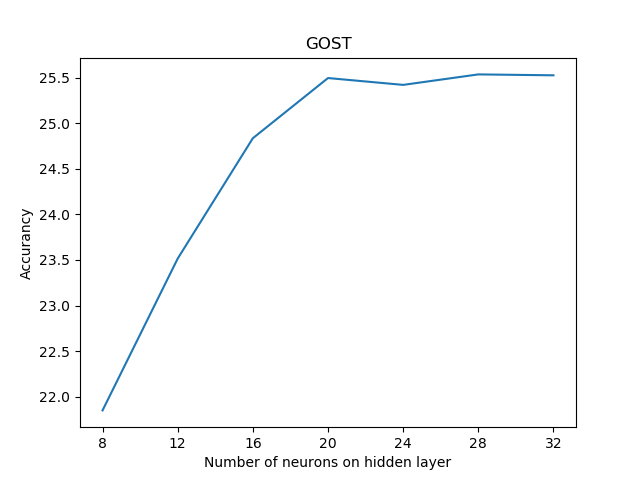
\includegraphics[width=0.9\linewidth]{report_1/acc_x_1.png}
	
	График точности построенной неройной сети от кол-ва нейронов на скрытом слое.
	\end{figure}
	
	\bigskip
	
	\noindent Данный метод показывает высокую точность и не требует больших вычислительных ресурсов, как в случае с построением нейронной сети для однотактового преобразования шифрования ГОСТ 28147-89.
	
	\newpage	
	\section*{Литература}
	\bigskip
	\begin{enumerate}
		\item Харин Ю.С., Берник В.И., Матвеев Г.В., Агиевич С.В. Математические и компьютерные основы криптологии. — 2003. — Минск.
		\item Neural networks in cryptography [Электрон. ресурс]. — 2015. — \\
		$\underline{http://cryptowiki.net/index.php?title=Neural\_networks\_in\_cryptography}$.
		\item Pattanayak S., Ludwig S.A. Encryption based on Neural Cryptography. — 2017.
		\item Kinzel F., Kanter I. Neural Cryptography. — 2002.
	\end{enumerate}
	
\end{document}